\documentclass[12pt,twoside]{report}

% some definitions for the title page
\newcommand{\reporttitle}{asdfasdf}
\newcommand{\reportauthor}{Your name}
\newcommand{\supervisor}{Name of supervisor}
\newcommand{\reporttype}{Type of Report/Thesis}
\newcommand{\degreetype}{Type of degree} 

% load some definitions and default packages
%%%%%%%%%%%%%%%%%%%%%%%%%%%%%%%%%%%%%%%%%
% University Assignment Title Page 
% LaTeX Template
% Version 1.0 (27/12/12)
%
% This template has been downloaded from:
% http://www.LaTeXTemplates.com
%
% Original author:
% WikiBooks (http://en.wikibooks.org/wiki/LaTeX/Title_Creation)
%
% License:
% CC BY-NC-SA 3.0 (http://creativecommons.org/licenses/by-nc-sa/3.0/)
% 
%
%%%%%%%%%%%%%%%%%%%%%%%%%%%%%%%%%%%%%%%%%
%----------------------------------------------------------------------------------------
%	PACKAGES AND OTHER DOCUMENT CONFIGURATIONS
%----------------------------------------------------------------------------------------
\usepackage[a4paper,hmargin=2.8cm,vmargin=2.0cm,includeheadfoot]{geometry}
\usepackage{textpos}
\usepackage{natbib} % for bibliography
\usepackage{tabularx,longtable,multirow,subfigure,caption}%hangcaption
\usepackage{fancyhdr} % page layout
\usepackage{url} % URLs
\usepackage[english]{babel}
\usepackage{amsmath}
\usepackage{graphicx}
\usepackage{dsfont}
\usepackage{epstopdf} % automatically replace .eps with .pdf in graphics
\usepackage{array}
\usepackage{latexsym}
\usepackage[pdftex,hypertexnames=false,colorlinks]{hyperref} % provide links in pdf

\hypersetup{pdftitle={},
  pdfsubject={}, 
  pdfauthor={},
  pdfkeywords={}, 
  pdfstartview=FitH,
  pdfpagemode={UseOutlines},% None, FullScreen, UseOutlines
  bookmarksnumbered=true, bookmarksopen=true, colorlinks,
    citecolor=black,%
    filecolor=black,%
    linkcolor=black,%
    urlcolor=black}

\usepackage[all]{hypcap}


%\usepackage{color}
%\usepackage[tight,ugly]{units}
\usepackage{float}
\usepackage{amsfonts}
%\usepackage{tcolorbox}
%\usepackage[colorinlistoftodos]{todonotes}
% \usepackage{ntheorem}
% \theoremstyle{break}
% \newtheorem{lemma}{Lemma}
% \newtheorem{theorem}{Theorem}
% \newtheorem{remark}{Remark}
% \newtheorem{definition}{Definition}
% \newtheorem{proof}{Proof}


%%% Default fonts
\renewcommand*{\rmdefault}{bch}
\renewcommand*{\ttdefault}{cmtt}



%%% Default settings (page layout)
\setlength{\parindent}{0em}  % indentation of paragraph

\setlength{\parindent}{0em}  % indentation of paragraph

\setlength{\headheight}{14.5pt}
\pagestyle{fancy}
\renewcommand{\chaptermark}[1]{\markboth{\chaptername\ \thechapter.\ #1}{}} 
%\fancyhead[RO]{\sffamily \textbf{\thepage}} %Page no.in the right on even pages
%\fancyhead[LE]{\sffamily \textbf{\thepage}} %Page no. in the left on odd pages

\fancyfoot[ER,OL]{\thepage}%Page no. in the left on
                                %odd pages and on right on even pages
\fancyfoot[OC,EC]{\sffamily }
\renewcommand{\headrulewidth}{0.1pt}
\renewcommand{\footrulewidth}{0.1pt}
\captionsetup{margin=10pt,font=small,labelfont=bf}


%--- chapter heading
\def\@makechapterhead#1{%
  \vspace{10\p@}%
  {\parindent \z@ \raggedright \sffamily
    \interlinepenalty\@M
    \Huge\bfseries \thechapter \space\space #1\par\nobreak
    \vskip 30\p@
  }}
%--- chapter heading
\def\@makechapterhead#1{%
  \vspace{10\p@}%
  {\parindent \z@ \raggedright \sffamily
        %{\Large \MakeUppercase{\@chapapp} \space \thechapter}
        %\\
        %\hrulefill
        %\par\nobreak
        %\vskip 10\p@
    \interlinepenalty\@M
    \Huge\bfseries \thechapter \space\space #1\par\nobreak
    \vskip 30\p@
  }}
%---chapter heading for \chapter*  
\def\@makeschapterhead#1{%
  \vspace*{10\p@}%
  {\parindent \z@ \raggedright
    \sffamily
    \interlinepenalty\@M
    \Huge \bfseries  #1\par\nobreak
    \vskip 30\p@
  }}    
\allowdisplaybreaks


\usepackage{titlesec}
\titleformat{\chapter}[hang]
  {\normalfont\huge\bfseries}{\thechapter\space\space}{0pt}{}
\titlespacing*{\chapter}{0pt}{0pt}{10pt}

\makeatletter
\renewcommand\chapter{\clearpage
                    \thispagestyle{plain}%
                    \global\@topnum\z@
                    \@afterindentfalse
                    \secdef\@chapter\@schapter}
\makeatother

% load some macros
% Here, you can define your own macros. Some examples are given below.

\newcommand{\R}[0]{\mathds{R}} % real numbers
\newcommand{\Z}[0]{\mathds{Z}} % integers
\newcommand{\N}[0]{\mathds{N}} % natural numbers
\newcommand{\C}[0]{\mathds{C}} % complex numbers
\renewcommand{\vec}[1]{{\boldsymbol{{#1}}}} % vector
\newcommand{\mat}[1]{{\boldsymbol{{#1}}}} % matrix


% load title page
\begin{document}
% Last modification: 2015-08-17 (Marc Deisenroth)
\begin{titlepage}

\newcommand{\HRule}{\rule{\linewidth}{0.5mm}} % Defines a new command for the horizontal lines, change thickness here

%----------------------------------------------------------------------------------------
%	LOGO SECTION
%----------------------------------------------------------------------------------------


\includegraphics[width = 4cm]{./figures/imperial}\\[0.5cm] 

\center % Center everything on the page
 
%----------------------------------------------------------------------------------------
%	HEADING SECTIONS
%----------------------------------------------------------------------------------------

\textsc{\LARGE MSc Computing Dissertation}\\[1.5cm] 
\textsc{\Large Department of Computing}\\[0.5cm] 
\textsc{\large Imperial College of Science, Technology and Medicine}\\[0.5cm] 

%----------------------------------------------------------------------------------------
%	TITLE SECTION
%----------------------------------------------------------------------------------------

\HRule \\[0.4cm]
{ \huge \bfseries Topology of Language for Semantic Entailment - Background Report v1}\\ % Title of your document
\HRule \\[1.5cm]
 
%----------------------------------------------------------------------------------------
%	AUTHOR SECTION
%----------------------------------------------------------------------------------------

\begin{minipage}{0.4\textwidth}
\begin{flushleft} \large
\emph{Author:}\\
Alexander Harrison Bull % Your name
\end{flushleft}
\end{minipage}
~
\begin{minipage}{0.4\textwidth}
\begin{flushright} \large
\emph{Supervisor:} \\
Tolga Birdal % Supervisor's Name
\end{flushright}
\end{minipage}\\[4cm]




%----------------------------------------------------------------------------------------


%----------------------------------------------------------------------------------------
%	DATE SECTION
%----------------------------------------------------------------------------------------

{\large \today} % Date, change the \today to a set date if you want to be precise


\vfill % Fill the rest of the page with whitespace
Submitted in partial fulfillment of the requirements for the MSc Computing of Imperial College London

\end{titlepage}



% page numbering etc.
\pagenumbering{roman}
\clearpage{\pagestyle{empty}\cleardoublepage}
\setcounter{page}{1}
\pagestyle{fancy}

%%%%%%%%%%%%%%%%%%%%%%%%%%%%%%%%%%%%
\newpage
\vspace*{-\fill}
\begin{abstract}
Semantic entailment, the question of whether a hypothesis $h$, can be inferred from a text $t$, is a core part of the field of Natural Language Processing (NLP), and one that is key to many important tasks including ``QA [question answering], IR [information retrieval], text summarization, machine translation, information extraction, and paraphrasing.'' \cite{PARAMASIVAM20229644} 
\newline \par
Semantic entailment is also a fundamental task for large language models (LLMs), on which many people are beginning to rely on for knowledge on a daily basis, thus becoming an ever more integral part of society. It is evident that for LLMs to provide reliable, robust answers to questions and meet the expectations of users, an ability to accurately understand questions of semantic entailment is crucial. Yet, given the fact that LLMs are often ``trained on text alone, without additional grounding,'' \cite{merrill-etal-2022-entailment} where training objectives focus on predicting missing words, many argue that this ``language modelling task, because it only uses form as training data, cannot in principle lead to learning of meaning.'' \cite{bender-koller-2020-climbing} \newline \par
In this thesis, we seek to bridge this gap and improve the performance and reliability of LLMs by imbuing them with the concept of semantic entailment during their training. We apply highly novel approaches for understanding semantic entailment through Topological Data Analysis (TDA) to study the topology of language, to develop a new metric that can robustly measure entailment, based theoretically on the concepts of entailment cones in hyperbolic geometric space. Subsequently, we mould the new entailment metric into a differentiable function that we inject as a regularizer into the training process of an LLM; where an additional optimization goal during the LLM's training is to maintain high entailment scores. We compare our `entailment-enhanced' LLM against various SOTA-models on core entailment challenges and demonstrate that our method results in an improvement of at least XX\% F1-score compared to the next best model, across all datasets. 



\end{abstract}


\section*{Acknowledgments}
Comment this out if not needed.

\clearpage{\pagestyle{empty}\cleardoublepage}

%%%%%%%%%%%%%%%%%%%%%%%%%%%%%%%%%%%%
%--- table of contents
\fancyhead[RE,LO]{\sffamily {Table of Contents}}
\tableofcontents 


\clearpage{\pagestyle{empty}\cleardoublepage}
\pagenumbering{arabic}
\setcounter{page}{1}
\fancyhead[LE,RO]{\slshape \rightmark}
\fancyhead[LO,RE]{}

%%%%%%%%%%%%%%%%%%%%%%%%%%%%%%%%%%%%
\chapter{Introduction}
\section{Motivation of the Thesis}
Language lies at the heart of the upsurge in Artifical Intelligence over the last 10 years. The arrival of Large Language Models (LLMs) like ChatGPT who can almost flawlessly reproduce language, discourse on any subject, and answer even the most complex of questions with relative assuredness has been transformative across industry and academia alike. Indeed, the prowess with which such LLMs have seemingly mastered language has led, particularly amongst mainstream media, to comparisons with ``god-like'' technology. \cite{hogarthFT} Investigations into the nature of language through the lens of topology, and the ability for LLMs to truly master language, form the core motivation for this thesis, which is discussed in the following section. 


\subsection{What is the meaning of language?}

Whilst this is a Computer Science thesis, and one that we believe will lead to significant novel discoveries that will materially improve the performance of LLMs in semantic entailment tasks, the fundamental motivation behind the topic is the same question that motivated my undergraduate dissertation in Modern and Medieval Languages; namely - what does it mean to \textbf{\textit{truly}} speak a language. \newline \par

I began that dissertation with a quote from Bertolt Brecht during his exile in the United States, that I believe is equally relevant for this thesis:
\begin{quote}
    I haven't the slightest hope of ever learning colloquial American English. It's certainly not for a lack of trying [...] It's something else that evades me. [...] In discussions, I'm not able to say what I want, just what I can. [...] One could assume that this confusing state would be temporary [...], but that is sadly wishful thinking. It's not that I'm unable to grasp the vocabulary, nor the syntactical or grammatical knowledge. Rather, what I cannot grasp is a certain linguistic \textit{Habitus}, which I simply do not see any possibility of learning.\cite{brecht}
\end{quote}

Brecht's experience of fluency of alienation from the linguistic \textit{habitus} of a foreign language, no matter how fluently it is spoken, is one that would resonate with any linguist. Yet, we ask and, indeed, expect LLMs to inhabit the linguistic \textit{habitus} of all languages at the same time with expert accuracy. \newline \par

In addition to an expectation of fluency and familiarity with our language, we also expect LLMs to understand and answer our questions in the same reasonable and reliable manner as we would expect from a subject matter expert. To fulfil these expectations, the ability for LLMs to understand semantic `meaning' and entailment is key. This is, however, not the case today. LLMs are commonly ``trained on text alone, without additional grounding''\cite{merrill-etal-2022-entailment}, with the missing-word prediction training tasks unable ``in principle [to] lead to learning of meaning.''\cite{bender-koller-2020-climbing} \newline \par 
While Bender et al. cast doubt on the ability of LLMs to truly understanding meaning, and hence to robustly evaluate more challenging semantic entailment tasks, these are also something that humans can often falter with. For example, given the premise ``All men are created equal'' with contextual knowledge of its origin in the US Declaration of Independence, multiple `valid' interpretations of the hypothesis ``Every person has the same inherent value'' are possible, each with very different ramifications:
\begin{enumerate}
    \item \textit{Contradiction}: `Men' in 1776 deliberately excluded women, enslaved people, Indigenous peoples.
    \item \textit{Entailment}: Despite historical limitations, the principle of the hypothesis is universal and should be understood as such.
\end{enumerate}

The inherently uncertain, fallible and \textit{individual} nature of language that these examples have attempted to exemplify is one best summarised by Jacques Derrida \cite{derrida1, derrida2, derrida3}, who maintains that the meaning of all language, whether speech or writing, is created through unstable, spatial and temporal relations between signifiers, that he terms différance - with every language-speaker caught up in the matrix of differences through which language functions. \newline \par

A core driver of this thesis then, is to investigate whether - contrary to the philosophical arguments given above - we can use concepts from the field of Topological Data Analysis to find an objective, \textit{universal} mathematical representation of language in which the concept of entailment can be robustly defined, modelled, and imbued into an LLM training regime, in order to improve its performance.


\subsection{The importance of understanding language in the age of Artificial Intelligence}
The questions raised in the previous section are of far greater practical significance than the intellectual curiosities that they may appear to be on the surface. Since the advent of LLMs only a few years ago, society has grown rapidly reliant on them - ChatGPT alone is forecast to have 1 billion users, almost 10\% of the world's population, by the end of 2025 at the latest. \cite{forbesChatGPT} \newline \par

Given this trajectory towards dependency on the outputs of LLMs, where such tools are consulted in the making of critical personal, business, or even political decisions, the safety and trustworthiness of LLM responses provided is of essential importance. Yet this is precisely where we have the least understanding and control of LLMs themselves. As explained by Fitz et al. (2024) \cite{fitz2024hiddenholestopologicalaspects}, ``as of now it is still a mystery why certain behaviours emerge in large language models, and little is understood about the structure of their representation manifolds.'' Many elements of how LLMs function still remain a `black box'. We interact with them at the level of their textual output, in which ``the natural topological structure of [the] language embeddings, which define the ``thoughts'' of the system, is lost'' \cite{fitz2024hiddenholestopologicalaspects}. For example, Figure 1.1, taken from Fitz (2022), \cite{fitz22a} shows a graph projection of vector space embeddings of word tokens from French and English. The differences in shape are striking, but the reasons for these differences are still unclear. \newline

\begin{figure}[tb]
\centering
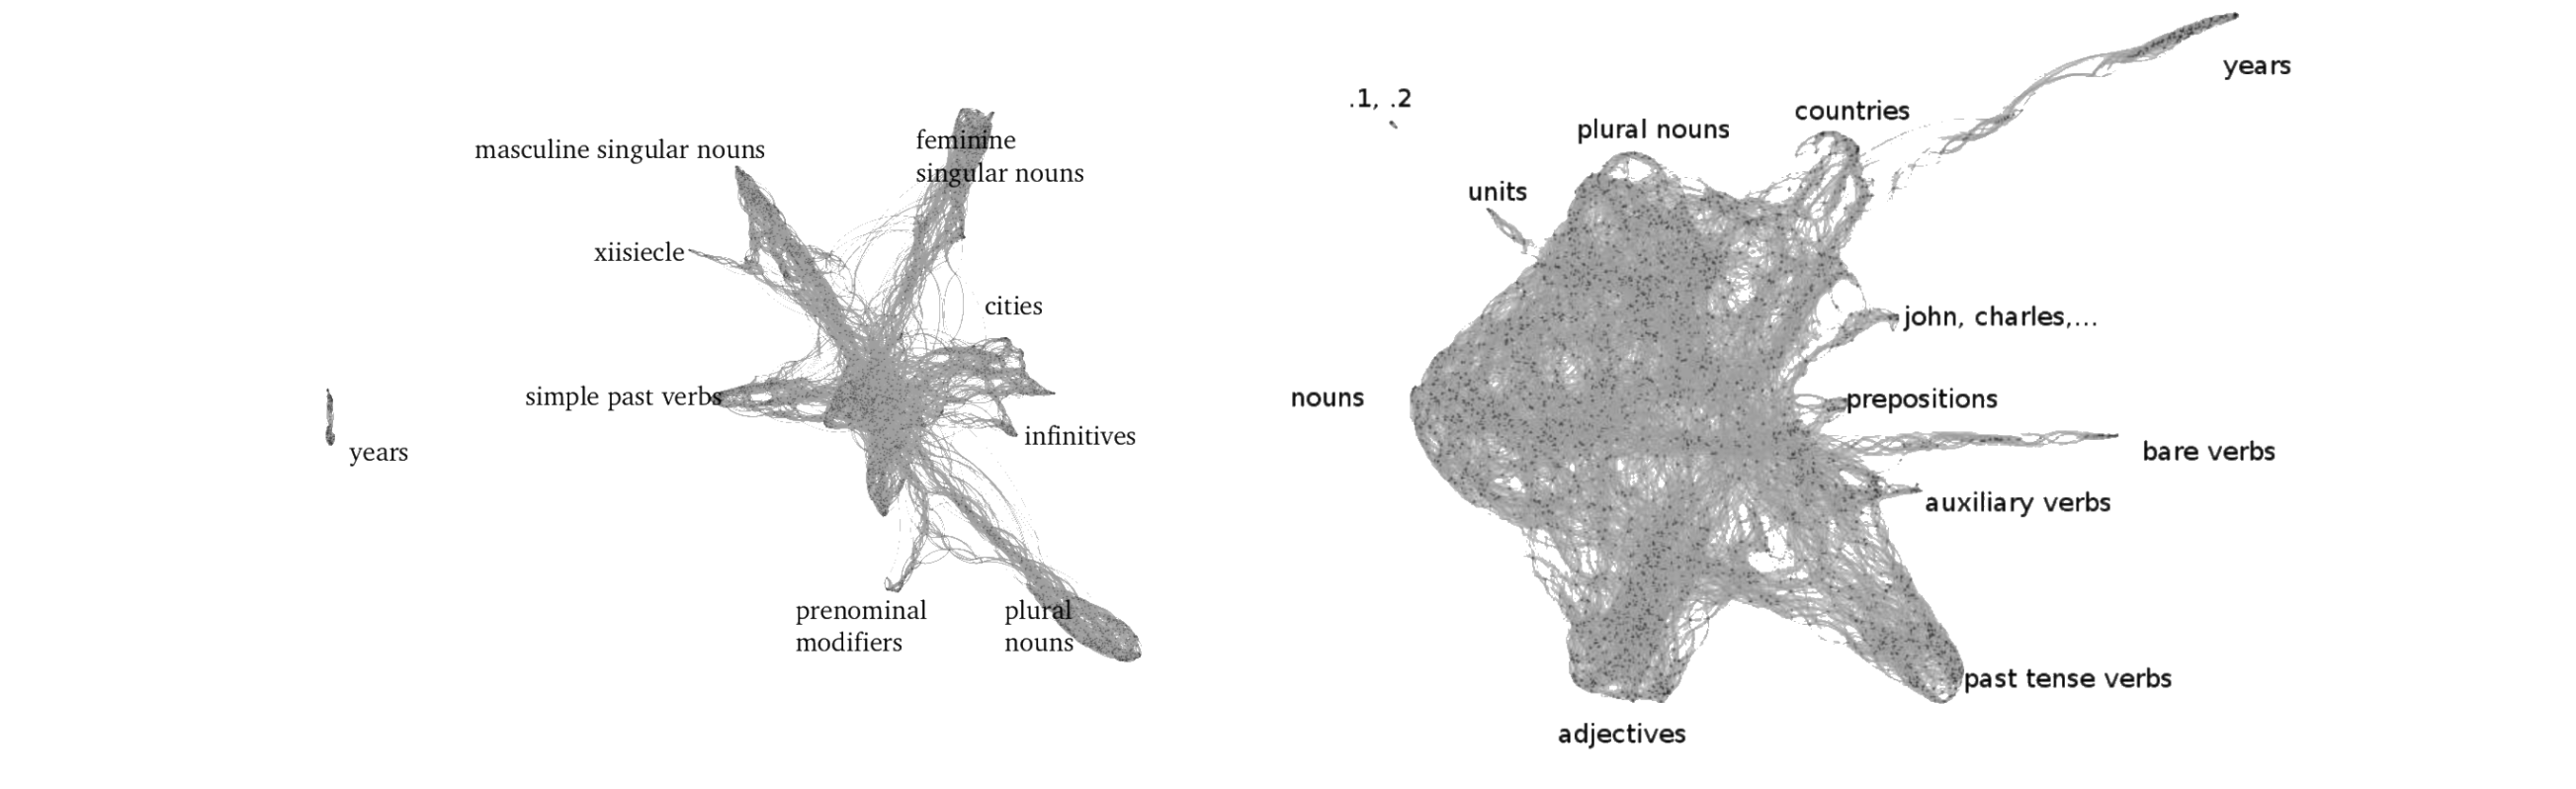
\includegraphics[width = 1\hsize]{./figures/graph_projection_fitz}
\caption{A graph projection of vector space embeddings of word tokens derived from corpora of French (left) and English (right).}
\label{fig:EmbeddingsFrenchEnglish}
\end{figure}

\par
This thesis hence seeks to conduct further investigations into the topology and geometry of the vector embeddings of language in LLMs. Such investigations are of manifold importance: the more we understand about the topology and geometry of LLMs, the better we can understand why they exhibit certain behaviours, and how we can improve their efficiency and parametrisation, potentially enabling smaller, more compressed models \cite{fitz2024hiddenholestopologicalaspects}. \newline \par

We, however, will focus specifically on understanding how relationships of semantic entailment are projected into the vector spaces that allow LLMs to `think'. We aim to develop an entailment metric that, when implemented as a regularizer in LLM training, will lead to better LLM performance on semantic entailment tasks. In doing so, we may also uncover potential answers to some of the more philosophical questions posed in the previous section, relating to what it means to speak a language, for humans and for AI. 

\section{Research Aim And Contributions}

The aim of this project is to understand the topology of language in LLM vector spaces and derive therefrom a robust expression that characterises the notion of semantic entailment, which, when used as a regularizer in LLM training, can improve performance on semantic and visual entailment tasks.  \newline \par

To achieve this aim, we make the following contributions: 

\begin{enumerate}
    \item \textbf{We implement topological data analysis (TDA) techniques (persistent homology, MAPPER) to investigate topological relationships between entailed, contradictory, and neutral premise-hypothesis pairs.} In Chapter X, we undertake this for semantic entailment, using the Stanford Natural Language Inference (SNLI) dataset. In Chapter (X+1), we replicate this task for a visual entailment dataset (SNLI-VE), where premises are given in the form of images rather than phrases.
    \item \textbf{We develop a robust mathematical expression for entailment using concepts from hyperbolic geometry - namely hyperbolic entailment cones}, from which we derive an entailment metric that can produce accurate entailment scores across semantic and visual entailment challenges; and be used to compare existing LLM performances on such tasks
    \item \textbf{We train an LLM with an `entailment regularizer'}, based on the entailment expression in 2., and demonstrate that it has superior performance on semantic and visual entailment tasks vs. SOTA benchmarks 
    \item \textbf{We reason briefly on the philosophical and linguistic implications of our findings}, including what our findings imply about linguistic theories such as Chomsky's universal grammar. 
\end{enumerate}


\section{Report Structure}
Chapter 2 provides an overview of the relevant theoretical and practical background to this work. This includes an outline of the logic and theory underpinning questions of entailment (Section 2.1), and a survey of major existing approaches to both semantic and visual entailment within the fields of NLP and computer vision, respectively (Section 2.2). We also provide a brief grounding in key concepts from Topological Data Analysis (TDA) and hyperbolic geometry for the unfamiliar reader (Section 2.3), and highlight the handful of existing  applications of TDA to language and LLMs, upon which this thesis builds. \par   \quad In Chapter 3, we develop the core theoretical element of this thesis, introducing the topological mapping of premise-hypothesis pairs, and the development of a metric to measure semantic entailment. \par 
\quad Chapter 4 presents experimental results displaying the robustness of the entailment metric across both semantic and visual entailment datasets, and evaluates the performance of SOTA LLMs to detect entailment, compared to our metric. \par
\quad Chapter 5 outlines the approach taken to extend our expression for entailment into a differentiable function that we implement as a regularizer in the training of an LLM, and demonstrates, through experiments, its superior performance against both SOTA LLMs, and other benchmark methods used in entailment challenges. \par
\quad Finally, Chapter 6 summarizes the contributions of this thesis, discusses potential avenues for future work suggested by our findings, and attempts to provide an answer to some of the more philosophical and linguistic questions raised by this research before concluding the thesis.




%%%%%%%%%%%%%%%%%%%%%%%%%%%%%%%%%%%%
\chapter{Background and Related Work}
This chapter presents an overview of existing progress and key related works in the fields of semantic and visual entailment, before providing a minimum theoretical grounding in the primary Topological Data Analysis (TDA) and Hyperbolic Geometry methodologies that will be used throughout this thesis. \newline \par

Section 2.1 focuses on logical representations of entailment tasks, which help to provide the theoretical framework for how we practically apply topological data analysis (TDA) methods in this thesis. \par \quad Section 2.2 introduces key practical datasets that have been used to experiment with semantic and visual entailment challenges in the NLP and Computer Vision communities respectively, alongside the metrics used, and varying approaches that have already been adopted.  \par \quad Finally, section 2.3 introduces two key Topological Data Analysis (TDA) methodologies - Persistent Homology and MAPPER - before discussing their relevance to language through exploring theoretical papers relating to the geometry of language. Section 2.3 closes by surveying existing practical applications of TDA in NLP, before briefly discussing the benefits of Euclidean vs. Hyperbolic Geometry in the context of semantic entailment - a question that is highly relevant for the practical approach we decide to adopt in the following chapters of this thesis. 

\section{Logical Representations of Entailment}

This thesis is an investigation of the Topology of Language for Semantic Entailment in the context of LLMs and, naturally, this was the focus of the introduction in Chapter 1. But to understand how semantic entailment can be captured through topological methods, we first need to examine its foundations in formal logic. Semantic entailment is, of course, fundamentally an exercise in logic. Natural language sentences can be broken down into their fundamental logical constituents and evaluated in Conjunctive Normal Form (CNF) through the language of propositional or predicate logic - and indeed this is one of the existing approaches to Semantic Entailment tasks that will be outlined in Section 2.2. As a simple example \cite{fSadri}, take the premises: 
\begin{flushleft}
\text{`If there are national elections, either the Tory party wins or the Labour party wins.'} \\
\text{`If the unions do not support the Labour party then it does not win.'} \\
\text{`There are national elections.'}

\end{flushleft}

\par and the hypothesis:
\begin{flushleft}
If the Tory party does not win then the unions
support the Labour party?    
\end{flushleft}

Using `E' to stand for elections, `L' to stand for a Labour victory, `T' to stand for a Tory victory, and `U' to stand for unions supporting labour, we can easily remodel these natural language statements into CNF: \newline 
\begin{align*}
\text{Premise:} \quad & E \rightarrow L \lor T, \quad \lnot U \rightarrow \lnot L, \quad E \\
\text{Conclusion:} \quad & \lnot T \rightarrow U
\end{align*}

From which we can easily prove that the conclusion is entailed by the premise, since in all cases where $\lnot T$ is true, we can see from the first WFF of the premise that $L$ must be true, and hence from the second that $U$ must also be true. \newline \par

This relationship between semantic entailment and logical entailment is important, because multiple works have derived `idioms' of entailment from logical analysis, which, as we shall now outline, provide justification for this thesis' hypothesis that topological features in embedding spaces can capture semantic entailment relationships. 

\subsection{Entailment as a Subsumption Relationship of Hypergraphs}

Jennings et al. \cite{leibnizianAnalysis} formulate a novel approach to entailment, using Leibnizian analysis to demonstrate how logic entailment can be demonstrated through subsumption relationships between hypergraphs. Before discussing their work and its relevance to this thesis, we first outline several key concepts for the unfamiliar reader: \newline
\begin{itemize}
    \item \textbf{Possible Worlds}. In logic, a possible world represents one possibility of truth values. For example, if we have a simple logical premise represented by literals $p$ (meaning, say, that it is raining), and $q$ (meaning, say, that the ground is wet), there are four possible worlds:
    \begin{enumerate}
        \item $w_1$: both p and q are true
        \item $w_2$: p is true, q is false
        \item $w_3$: p is false, q is true
        \item $w_4$: both p and q are false
    \end{enumerate}
    \item \textbf{Powersets}. The powerset of possible worlds, denoted by Jennings et al. as $\wp(U)$ \cite{leibnizianAnalysis}, is the set of all possible sets, i.e. representing the universe in a full propositional model. The subset $\{w_1, w_2\}$ within $\wp(U)$ would, in this example, represent all worlds in which ``it is raining'' is true. 
    \item \textbf{Hypergraphs}. Borrowing the defintion directly from Jennings et al. \cite{leibnizianAnalysis}, ``a hypergraph $H$ is a pair $H=(X, E)$ where $X$ is a set of elements, called nodes or vertices, and $E$ is a non-empty set of non-empty subsets of $X$, each of which is called a (hyper-)edge. [...] Conventionally, we can write $H$ as a collection of edges, i.e. $H=\{E_1, E_2, ..., E_n\}$, where $\forall i, 1 \leq i \leq n, E_i \in X$. 
    \item \textbf{Atomic Constituents}. An atomic constituent is the simplest, irreducible form of a logical expression - i.e., a literal in propositional logic. By this definition CNF can be viewed as a disjunction of atoms.
\end{itemize}

With this background, we can summarize the key insights outlined by Jennings et al. \cite{leibnizianAnalysis}, and their relevance for a topological investigation of semantic entailment in this thesis. We refer the interested reader to \cite{leibnizianAnalysis} for the mathematical proofs of these insights. \newline \par \quad 
1. Since `every sentence has a finite analysis into its conjunctive normal form [...], semantically, then, every sentence of that language can be represented as a simple hypergraph, $H$, on the powerset of a universe of states'. \newline \par
This is particularly relevant in the context of this thesis' topological approach, since hypergraph representations can naturally embed logical relationships into a geometric form. \newline \par \quad
2. An entailment relationship $\alpha \models \beta$, corresponds to a subsumption relationship between two hypergraphs on $\wp(U)$, such that $H_{\alpha} \sqsubseteq H_{\beta}$. The subsumption relationship is defined as true if \cite{leibnizianAnalysis}: 
$$
\forall H, H' \in \mathbb{H},\; H \sqsubseteq H',
\text{ if and only if }
\forall E' \in H',\; \exists E \in H \text{ such that } 
\forall e \in E,\; \exists e' \in E' : e \leq e'  
$$ 

where $\mathbb{H}$ is a set of \textit{simple} hypergraphs such that $\mathbb{H} \subseteq \wp\wp(U)$. \newline \par

Figure 2.1 demonstrates a trivial example of this, where a premise $(p \lor q \lor r) \land (\neg s \lor q) $  is modelled by the hypergraph $H_A$, whilst a conclusion $q \lor r$ is modelled by hypergraph $H_B$.

\begin{figure}[H]
\centering
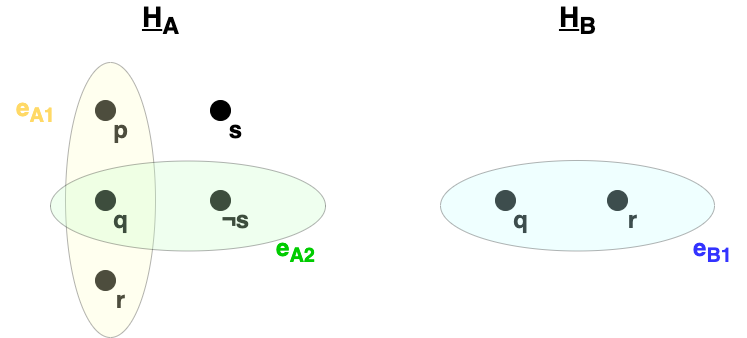
\includegraphics[width = 1\hsize]{./figures/HypergraphIntro.drawio.png}
\caption{A hypergraph representation of $(p \lor q \lor r) \land (\neg s \lor q)$ in $H_A$, and $q \lor r$ in $H_B$}
\label{fig:Hypergraphs}
\end{figure}

Following the definition given above, for the conclusion $H_B$ to be entailed by the premise $H_A$, every hyperedge of $H_B$ (in this case just $e_{b1}$), must be `underwritten' by at least one hyperedge in $H_A$. We can clearly see this is the not the case, and the conclusion is not entailed by the premise, since $H_A$ has no hyperedge containing just $\{q, r\}$. \newline

The entailment relationship described above is also highly relevant to this thesis, as it provides a theoretical foundation according to which we can look for entailment relationships in our topological investigations of language. \newline \par

\quad 3. The definition of entailment relationships via subsumption leads to the emergence of an algebraic lattice structure; namely that $\langle\mathbb{H}, \sqsubseteq\rangle$ is a lattice \cite{leibnizianAnalysis}. The connection between entailment relations and distributive lattices is further developed by Cederquist and Coquand \cite{Cederquist}, who establish a direct bridge between the abstract logical system of entailment relations and topological spaces, through the use of distributive and normal lattices. This lattice structure has the following important tenets:
\begin{enumerate}
    \item \textbf{Partial Order}: The subsumption relation creates a partial order between the hypergraphs involved. For example, if $H_A \sqsubseteq H_B$, then we can colloquially think of $H_A$ as `containing more information' or being `higher' in the lattice than $H_B$
    \item \textbf{Lattice Operations}: Given any two hypergraphs $H_A$ and $H_B$, we can state that their \textit{join} $(H_A \lor H_B)$ is the hypergraph representing the weakest formula that \textbf{both entail}; whilst their \textit{meet} $(H_A \land H_B)$ is the hypergraph representing the strongest formula that \textbf{entails both}
    \item \textbf{De-Morgan Structure For Negation}: Logical negation can be accomplished using the blocker function $\tau$, which allows the following logical rules to hold true:
    \begin{itemize}
        \item $\tau(\tau(H_A)) = H_A$, i.e. double negation
        \item $H_A \sqsubseteq H_B \iff \tau(H_B) \sqsubseteq \tau(H_A)$, i.e. order reversal under negation
    \end{itemize}
\end{enumerate}

These findings are key for several reasons. Firstly, `the semantic idiom that hypergraph-theory affords reveals a hierarchy of lattices capable of representing entailments of every finite degree' \cite{leibnizianAnalysis}. Secondly, lattices themselves provide a bridge from discrete logical topographic structures (i.e. hypergraphs), to a continuous geometric space, where notions of `height' (how general vs. how specific a formula is), `distance' (how many steps in the lattice separate two formulae), and `directions' (moving up the lattice, as generalization, and moving down, as specialization) are all present. Combined, these two principles lay the theoretical foundation for this thesis' hypothesis that relationships of semantic entailment should be able to be detected and measured through topological analysis. The lattice structure should, in theory, enable the logical relationships of entailment to be preserved when we move from semantics in words and phrases across to their vector space embeddings in LLMs; while the partial order features of lattices capture the asymmetry of entailment, where $A \rightarrow B \neq B \rightarrow A$. \newline \par

The key insights from this brief theoretical overview of entailment is that entailment creates asymmetric, hierarchical structures - whether represented as:
\begin{itemize}
    \item Subsumption in hypergraphs (logical domain), as shown in \cite{leibnizianAnalysis}
    \item Partial orders in lattices (algebraic domain), demonstrated in \cite{Cederquist} and \cite{leibnizianAnalysis}
    \item Directional relationships in embeddings spaces (geometric domain), shown in Chapters 3 and 4
\end{itemize}


The topological approach this thesis takes aims to bridge these representations, drawing on the logical frameworks outlined above, while operating in the continuous, high-dimensional space of semantic embeddings in LLMs.


\subsection{From Logical to Semantic Entailment}

The theoretical and mathematical studies of entailment above focus on logical entailment. While logical entailment operates on formal symbols with fixed meaning, textual entailment in natural language - incorporating the lexical and syntactic meaning of words, phrases, and sentences - must grapple with the often ambiguous and context-dependent nature of language outlined in the introduction to this thesis. \newline \par

Some interesting work has already been undertaken studying the ability of neural networks and LLMs to tackle tasks involving logical entailment and textual entailment in natural language. Evans et al. \cite{Evans2018} developed a new neural network architecture termed a `PossibleWorldNet', that was able to achieve 96\% accuracy on tasks involving entailment in propositional logic. Such high performance suggested that the network was able to learn the structural patterns of entailment. As the authors state, for propositional logic, ``the problem of determining whether an entailment holds is a purely structural sequence-based problem: to evaluate whether an entailment is true, only the meaning of - or inference rules governing - the connectives is relevant. Everything else only has meaning via its place in the structure specified by an expression.'' \cite{Evans2018} \newline \par

The `PossibleWorldNet' architecture developed by Evans et al. is a variant of a TreeNet architecture that evaluates pairs of propositional logic formulae in different `possible worlds'. ``To evaluate whether $A \models B$, the PossibleWorldNet generates a set of imagined “worlds”, and then evaluates A and B in each of those worlds. It is a form of ``convolution over possible worlds'', [where] the quality of the model increases steadily as we increase the number of imagined worlds.'' \cite{Evans2018} This architecture significantly outperformed conventional architectures, such as transformers (by 40-50\%), and convolutional networks (by roughly 40\%). The authors suggest that the poor performance of these models is likely due to the inability to capture with sufficient precision the correct hierarchical structures that exist within logical expression. \newline \par

While these findings are strictly in the field of logical entailment, which ``unlike textual entailment, depends only on the meaning of logical operators, and of the place particular arbitrarily-named variables hold within a structure'' \cite{Evans2018}, these results do have an important implication for the textual entailment tasks we shall explore in this thesis. As is pointed out in \cite{Evans2018}, current neural models, including the transformer architecture that most LLMs are built on, can often fail to understand the structure of sentences they are meant to evaluate. For example, Bowman et al. \cite{bowman2015} demonstrate how all neural models they tested wrongly classified the premise ``\textit{A man wearing padded arm protection is being bitten by a German shepherd dog}'' and conclusion ``\textit{A man bit a dog}'' as an entailment relationship, instead of as a contradiction. Given this, Evans et al. emphasise the importance of ``isolating the purely structural sub-problems'' involved in questions of entailment, and claim that ``only networks that can reliably predict entailmetn in a purely formal setting, such as propositional (or first-order) logic, will be capable of getting these sorts of examples consistently correct.'' \cite{Evans2018}. This reinforces the importance of any entailment metric developed by this thesis to be built on the theoretical foundations of first-order logic, as is enabled by the lattice-based idiom of entailment that we explored in the previous section. \newline \par

Progressing from logical entailment to focus on natural language semantics, recent work by Merrill et al. \cite{merrill-etal-2022-entailment} explores whether LLMs could in principle learn \textit{meaning} and entailment semantics from being trained purely on text as they are today. They demonstrate that under highly specific conditions - namely when LLMs are trained on data generated solely by Gricean speakers who are ``uniformly truthful speakers'' and ``choose their utterances in order to balance two competing objectives: (a) conveying information to their listener and (b) brevity'' - then entailment relationships can be detected from this `ideal' language model's probability distributions. \newline \par

However, these conditions are often not representative of the average human speakers, and certainly not representative of the vast wealth of text that is available on the internet and that LLMs are trained on. It is hence no surprise, that the performance of LLMs, and of AI approaches in general, on tasks involving recognising textual entailment (RTE) leaves room for improvement. Indeed, in the survey of textual entailment based question answering methods, Paramasivam and Nirmala highlight that benchmark accuracy scores are often no higher than 50-70\%, particularly for generalised datasets with non-obvious hypothesis-premise entailment pairs that span across multiple domains \cite{PARAMASIVAM20229644}). 

\section{Progress, Approaches, and Benchmarks in Semantic and Visual Entailment}

\subsection{Recgonizing Textual Entailment (RTE)}

Recognizing Textual Entailment (RTE) is the common name given to the ``evaluation framework [used] to compare semantic understanding of different NLP systems,'' \cite{poliak-2020-survey} through testing their ability to determine if one sentence can be inferred from another. The definition of entailment used in RTE is more lenient than strict definition used in linguistics whereby ``sentence A entails sentence B if in all models in which the interpretation of A is true, also the interpretation of B is true.'' \cite{sep-montague-semantics} This difference is highlighted in the annotation guidelines of the 2005 PASCAL RTE dataset released by Dagan et al, in which is stated that, for the purposes of RTE, entailment means that ``in principle, the hypothesis must be fully entailed by the text. Judgement would be False if the hypothesis includes parts that cannot be inferred from the text. However, cases in which inference is very probable (but not completely certain) are still judged as True.'' \cite{dagan2005} \newline \par

This is an important distinction. The ``fuzzier notion of entailment'' \cite{poliak-2020-survey} used by RTE is highly indicative of the purpose of the RTE challenges - namely to evaluate the semantic understanding of NLP systems, which are built with specific objectives - be it as an LLM, a machine translator, an information retrieval system or otherwise. In virtually all these cases, where inference is very probable, it is beneficial for the system to evaluate the premise-hypothesis pair as entailed, (e.g. resulting in it retrieving the likely relevant information in the case where it is an IR system), rather than as contradictory. In a similar vein, we want NLP systems to be able to deal with cases of `near-contradiction' in NLP problems, such as in the example given by \cite{merrill-etal-2022-entailment}, where you have:
\begin{align*}
x =  \text{I’m not in North America}\\
y =  \text{I’m in a US state}    
\end{align*}

As Merril et al. point out, `$y$ nearly contradicts $x$ because they are both satisfiable only in worlds where the speaker is in Hawaii'', hence we need NLP systems to be able to judge whether $x$ and $y$ are entailed, contradictory, or neutral based on any additional context given. 

\subsection{Intrinsic vs. Extrinsic Evaluations}

In Poliak's survey on Recognizing Textual Entailment as an NLP Evaluation \cite{poliak-2020-survey}, he makes the helpful distinction between intrinsic evaluations, i.e. application-free and ``concerned with the system’s own objectives'' \cite{estival1997}, and extrinsic criteria, i.e. application-driven and ``concerned with the function of the system in relation to its set-up'' \cite{estival1997}. As a more concrete example, ``when evaluating a document summarization system, an intrinsic evaluation might ask questions related to the fluency or coverage of key ideas in the summary while an extrinsic evaluation might explore whether a generated summary was useful in a search engine.'' \cite{poliak-2020-survey} \newline \par

This is a helpful distinction to keep in mind as we provide an overview of the common approaches to RTE and key datasets used in RTE evaluations over the following sections; since an increasingly common criticism levelled against some of the common RTE datasets is a challenge to their ``ability to test the inferential capabilities of NLP models, [namely] a high accuracy on these datasets does not indicate which types of reasoning RTE models perform or capture.'' \cite{poliak-2020-survey} White et al. take this critique a step further, noting that ``researchers ompete on which system achieves the highest score on a test set, but this itself does not lead to an understanding of which linguistic properties are better captured by a quantitatively superior system.'' \cite{white-etal-2017-inference} Put differently, while the accuracy metric used to measure RTE does indicate how well a model determines if one sentence entails another, ``it does not illuminate how well NLP models capture different semantic phenomena that are important for general NLU.'' \cite{poliak-2020-survey} Through our topological approach to semantic entailment, we hope to not only improve the entailment accuracy on these RTE datasets, but also to be able to clearly define the topological features that can be used to robustly determine entailment.

\subsection{An Overview of Key RTE Datasets} 

The following section provides an overview of some of the key datasets that have been used either as training data to improve the ability of NLP systems to evaluate semantic entailment, or as test datasets to assess the abilities of such systems. Some of the datasets discussed below will be leveraged as training and test datasets for the experiments conducted in this thesis [add precisely which when experiments conducted]. \newline \par

\textbf{FraCas}. Developed by Cooper et al. in 1996 \cite{CooperFracas},   \textit{FraCas} is a short dataset of only about 350 examples of premise-hypothesis pairs, that were created manually by linguists, with the specific aim of testing an NLP systems' ability to understand a range of semantic phenomena including ``generalized quantifiers, plurals, anaphora, ellipsis, adjectives, comparatives, temporal references, verbs, and attitudes'' \cite{poliak-2020-survey}. Premises are at least one sentence long, but can be multiple, and hypothesis are written as a question, with possible answers being `\textit{Yes}' for entailment, `\textit{No}' for contradiction, or `\textit{Don't know}' for neutral. While the \textit{FraCas} dataset has the benefit of being crafted to evaluate an NLP systems' performance against specific semantic phenomena, its short size prevents it from being a viable model to train deep learning models on - although it remains useful as a test dataset. \newline \par

\textbf{Pascal RTE Challenges}. The first Pascal RTE challenge, developed by Dagan et al. \cite{dagan2005}, was designed as a generic evaluation framework ``to compare the inference capabilities of [NLP] models designed to perform different tasks.'' \cite{poliak-2020-survey}. It had more of a real-world applied focus than the \textit{FraCas} dataset, and hence hypothesis-premise pairs in the Pascal datasets were frequently taken from the downstream tasks of such sytems. For example, the first Pascal RTE dataset was extracted from ``7 tasks: comparable documents, reading comprehension, question answering, information extraction, machine translation, information retrieval, and paraphrase acquisition.'' \cite{poliak-2020-survey}. Since the first Pascal dataset in 2005, there have been eight further iterations, the most recent being Dzikovska et al. in 2013 \cite{dzikovska-etal-2013-semeval}. Examples of premise-hypothesis pairs from the first three Pascal iterations can be found in Table 1, taken from Poliak (p.5) \cite{poliak-2020-survey}. While the Pascal datasets are significantly larger than the \textit{FraCas} equivalents, they are still not of the size required to train deep learning models on - the first Pascal dataset, for instance, only contains roughly 1000 examples. This brings us onto the more recent, popular and larger RTE datasets that have largely been developed in order to train deep learning models.

\begin{figure}[H]
\centering
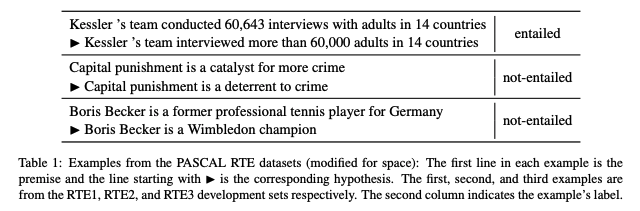
\includegraphics[width = 1\hsize]{./figures/PASCAL examples.png}
\label{fig:PASCAL}
\end{figure}

\textbf{Deep Learning Datasets}. We will briefly survey four key datasets that are large enough to be used as training datasets for deep learning models. The first of the four, \textit{Sentences Involving Compositional Knowledge} (SICK) was created in 2014 \cite{marelli-etal-2014-sick}, and contains roughly 10,000 examples that can be used to test semantic entailment (``with three possible labels: entailment, contradiction, and neutral'' \cite{PARAMASIVAM20229644}) and semantic similarity (via a 5 point scale rating). A year later, Bowman et al. \cite{bowman2015} created the \textit{Stanford Natural Language Inference} (SNLI) corpus, containing 570,000 examples of ``sentence pairs labelled for entailment, contradiction, and semantic independence.'' \cite{PARAMASIVAM20229644} In the SNLI corpus, the same premise can be paired with up to three different hypotheses, each with a potentially different entailment label, as displayed by Table 2 below, taken from Poliak (p.6)\cite{poliak-2020-survey}.


\begin{figure}[H]
\centering
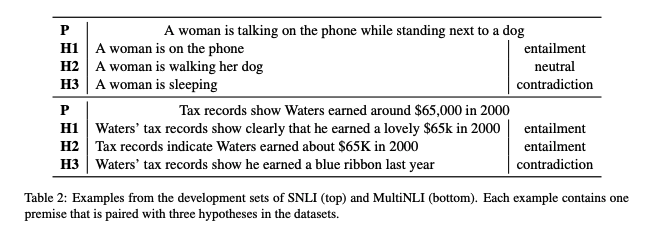
\includegraphics[width = 1\hsize]{./figures/SNLI examples.png}
\label{fig:SNLI}
\end{figure}

The \textit{Multi-Genre Natural Language Inference} (MNLI) dataset was introduced in 2018 by Williams et. al \cite{williams-etal-2018-broad}, to build on the SNLI dataset by collecting roughly 430,000 examples across ten different written and spoken languages, as opposed to SNLI where all examples are in English. The final dataset worth mentioning here is the \textit{SciTail} dataset developed by Khot et al. \cite{Khot_Sabharwal_Clark_2018}, which differs from the the three previously mentioned datasets, insofar as it is the only one of the four to have been created from existing textual sources, rather than through crowd-sourced workers and volunteers. The SciTail dataset is, however, a lot smaller than SNLI and MNLI, containing just under 30,000 examples of science-themed premise-hypothesis pairs. \newline \par


\subsection{Common approaches to semantic entailment tasks}

This section outlines the core approaches that have thus far been adopted to tackle textual entailment challenges, and highlights certain shortcomings and limitations of each approach. \newline \par

Following Paramasivam and Nirmala \cite{PARAMASIVAM20229644}, we categorise approaches to RTE as typically falling into one or several of the following categories:
\begin{itemize}
    \item \textbf{Lexical approaches}, that focus on the linguistic information of input surface strings, without considering syntactic or semantic properties
    \item \textbf{Semantic approaches}, which consider the meaning of the text in broader context to evaluate entailment, as opposed to only considering the input surface strings as in the lexical approach
    \item \textbf{Logical approaches}, where a logical representation language is used to determine entailment
    \item \textbf{AI approaches}, where entailment models are built to recognize entailment, with classifiers used to determine if a text-hypothesis pair of inputs results in entailment 
\end{itemize}

The shortcomings of solely \textbf{lexical} or \textbf{semantic} approaches are evident, since to understand meaning in any language, an understanding of both the lexis and syntax of the language is essential. Without an understanding of the broader context of the subject matter being discussed, lexical and syntactical understanding even together are still often not enough. Hence, a successful approach would require components of both the lexical and semantic approaches described above. However, major limitations still surround such approaches. Taking Shajalal et al's \cite{shajalal} approach as exemplary of this genre of RTE approaches, where they propose a methodology that converts into vector representation both lexical and semantic features of words, before using an average of the element-wise Manhattan distance vector (EMDV), Bag-of-Words based (BoW) similarity score, Jaccard similarity score (JAC), and the BERT-based semantic textual similarity score to determine entailment. The problem with this and similar lexical and/or semantic approaches is that they are measuring \textit{semantic similarity} to recognize \textit{semantic entailment}, when in reality, the two are in no way equal. \newline \par

Taking an example of the sentence pair:
\begin{flushleft}
    \textbf{Sentence A:} ``The cat is sleeping on the sofa''\\
    \textbf{Sentence B:} ``The dog is sleeping on the sofa''. 
\end{flushleft}

Both these sentences would result in high Bag-of-Words and Jaccard similarity scores, due to the fact that they share every word except for cat and dog. Similarly, in the majority of vector embeddings (such as BERT and Word2Vec), `cat' and `dog' are close neighbours from a distance perspective, due to their distributional similarity in training data. In the above sentences, they also play the same grammatical role as the subject of the sentence. Given this trivial example, we can already see how methods that rely on semantic similarity to measure entailment might falsely detect entailment where there is none (as could be the case in the above situation), and vice-versa. A further issue with purely distance-based methods is their inability to take into account the asymmetrical and hierarchical nature of entailment, that we discussed in section 2.1. This is again easily demonstrated by means of example:
\begin{flushleft}
    \textbf{Pair A:} \textit{Premise}: `All cats are animals'. \textit{Hypothesis}: `Some cats are animals' \\
    \textbf{Pair B:} \textit{Premise}: `Some cats are animals'. \textit{Hypothesis}: `All cats are animals'
\end{flushleft}

Given the premise and hypothesis in both pairs are identical, it is easy to see that a purely distance-based approach to entailment would fail to differentiate between the fact that \textit{Pair A} is an entailment relationship, while \textit{Pair B} is not an entailment relationship, because the directional relationship from specialisation to generalisation is going the wrong way. \newline \par

Purely \textbf{logical approaches} to entailment, such as the one discussed in Section 2.1.2 are able to resolve some of these difficulties due to their ability to focus on the structure and hierarchical relationships of arbitrarily-named variables; rather than having to deal with lexical and syntactical parsing of natural language. However, they are of less use for the purposes of this thesis, which focuses on developing a metric for semantic entailment that can be used to measure and improve the performance of LLMs. Given this context, an approach to semantic entailment that works in natural language, where words can be replaced by synonyms, and word order and syntax can be restructured without changing meaning, is essential. \newline \par

The category of \textbf{AI approaches} described by Paramasivam and Nirmala \cite{PARAMASIVAM20229644} is a broad one, and is mostly used to designate deep learning entailment models that may focus to greater or lesser on lexical, semantic or logical elements of sentences depending on the model. As Poliak notes \cite{poliak-2020-survey}, the recent advances in deep learning have led to ``a resurgence of interest in RTE amongst NLP researchers'' (p.6). Indeed, one needs to only look at the SNLI leaderboard to see the high accuracy scores that have been achieved with such AI approaches - with the current leading benchmark having achieved 94.7\% accuracy. Despite such high accuracy scores, these AI approaches also suffer from important shortcomings. As Poliak points out \cite{poliak-2020-survey}, the resurgence of deep learning approaches to RTE ``did not primarily focus on using RTE as a means to evaluate NLP systems. Rather, researchers primarily used these datasets to compete with one another to achieve the top score on leaderboards for new RTE datasets.'' (p.6) Going further than this, Pavlick argues that the high scores achieved in some of these leaderboards actually provide ``little evidence to suggest [that RTE models] capture the type of compositional or world knowledge tested by datasets like the FraCas test suits,'' \cite{pavlick2017} which were deliberately crafted in a manner to challenge the ability of NLP systems to cope with a range of semantic phenomena. Further evidence that this is the case is provided by Sanwal \cite{sanwal2024evaluatinglargelanguagemodels}, who showed how an LLM-based model that achieved 89.9\% accuracy on the SNLI dataset experienced a significant performance drop of 17\%, to only achieve 72.5\% accuracy when tested on a `contrast set'. Sanwal suggests that this drop in performance was likely due to limitations of the SNLI dataset which lacks the nuanced and diverse examples that were integrated to their contrast set, and were deliberately created to expose the model to a ``broader spectrum of linguistic scenarios.'' (p. 2) \newline \par

In summary, material shortcomings currently exist with every major category of approach to RTE tasks. While more recently `AI approaches' have yielded high accuracy scores on key datasets such as SNLI, their ability to generalise away from the often simple examples of these datasets is under scrutiny. By developing a metric for semantic entailment that is built upon solid logical and theoretical foundations, and that is demonstrable through topological data analysis, we seek to address some of these shortcomings since such a metric would:
\begin{itemize}
    \item Measure semantic entailment, rather than semantic similarity
    \item Be robust enough to deal with entailment examples that involve more nuanced linguistic phenomena 
\end{itemize}

\subsection{Visual Entailment}

Alongside semantic entailment sits the related task of visual entailment. Instead of a textual premise-hypothesis pair, in visual entailment tasks the premise is an image, while hypotheses remain textual sentences that models are to classify with \textit{entailment}, \textit{contradiction}, or \textit{neutral} labels. \newline \par

The key visual entailment dataset, \textit{SNLI-VE}, was developed by Xie et al.\cite{xie2019visualentailmentnoveltask} in 2019, and - as the name suggests - is built on the SNLI dataset discussed above. Figure 2.2, taken from Xie et al. (p. 2) \cite{xie2019visualentailmentnoveltask} provides an example of the premise-hypothesis pairs from SNLI-VE. 

\begin{figure}[H]
\centering
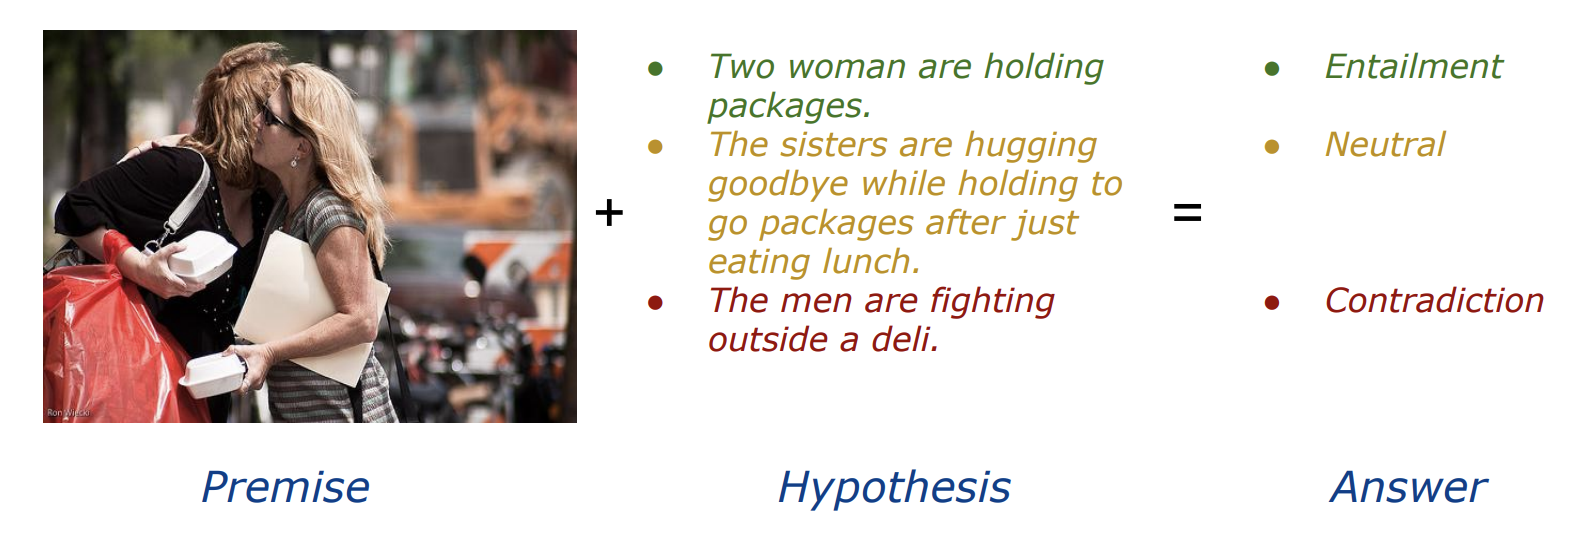
\includegraphics[width = 1\hsize]{./figures/SNLI-VE.png}
\caption{An Example from SNLI-VE dataset}
\label{fig:SNLI-VE}
\end{figure}

In the same paper, Xie et al. propose both transformer and CNN-based architectures as viable solutions to tackle the visual entailment challenge, achieving benchmark accuracy scores of just over 70\%.

The visual entailment task is of relevance to this thesis because we hypothesise that the topological entailment relationship we seek to define between textual premise-hypothesis pairs in a high-dimensional embedding space could also hold for multimodal premise-hypothesis pairs, where an image serves as the premise and text as the hypothesis. This would require mapping both visual and textual representations into a shared embedding space, enabling the hyperbolic entailment cone framework, that we seek to develop to describe entailment relationships, to operate across modalities.

\section{Topology of Language}
Theoretical approaches followed by  practical?
\subsection{Topological Data Analysis (TDA)}
\subsubsection{Persistent Homology}
\subsubsection{MAPPER}
\subsection{TDA applied to Language}
\subsubsection{Fractal Geometry of Language}
\subsubsection{Intrinsic Dimensionality}
\subsubsection{Practical Applications of TDA in NLP}
\subsection{Euclidean vs. Hyperbolic Geometry for Entailment Mappings}



%%%%%%%%%%%%%%%%%%%%%%%%%%%%%%%%%%%
\chapter{Project Plan}
Chapter for Background Interim Report only, for second marker feedback




%%%%%%%%%%%%%%%%%%%%%%%%%%%%%%%%%%%%
\chapter{Approach, 
Experimental Setup and Method}


%%%%%%%%%%%%%%%%%%%%%%%%%%%%%%%%%%%%
\chapter{Experimental Results and Discussion}
The results are very interesting in Jones 2019.

%%%%%%%%%%%%%%%%%%%%%%%%%%%%%%%%%%%%
\chapter{Conclusion}


%% bibliography
\bibliographystyle{unsrt}
\bibliography{References}

%%%%%%%%%%%%%%%%%%%%%%%%%%%%%%%%%%%%
\chapter*{Declarations}




\end{document}